\documentclass{article}
\usepackage[T1]{fontenc}
\usepackage{icml2026}
\usepackage{microtype}
\usepackage{graphicx}
\usepackage{booktabs}
\usepackage{colortbl}
\definecolor{hnegray}{gray}{0.93}
\usepackage{amsmath,amssymb}
\usepackage{hyperref}
\usepackage{stfloats}
\usepackage[section]{placeins}
\hypersetup{colorlinks=true,allcolors=black,pdftitle={HNE: Shared Representations for Early Warning of Rhythm Disruptions}}
\icmltitlerunning{HNE: Early Warning of Rhythm Disruptions}
\setcounter{topnumber}{2}
\setcounter{bottomnumber}{2}
\setcounter{totalnumber}{4}
\setcounter{dbltopnumber}{2}
\renewcommand{\topfraction}{0.85}
\renewcommand{\dbltopfraction}{0.7}
\renewcommand{\textfraction}{0.15}
\renewcommand{\floatpagefraction}{0.8}
\renewcommand{\dblfloatpagefraction}{0.8}
\newcommand{\hnetable}[1]{\begingroup\small\setlength{\tabcolsep}{3pt}\begin{minipage}{0.98\linewidth}\centering\input{#1}\end{minipage}\endgroup}
\newcommand{\emptyframe}[2]{\begingroup\setlength{\fboxsep}{0pt}\fbox{\rule{0pt}{#2}\rule{\dimexpr#1-2\fboxrule\relax}{0pt}}\endgroup}

\begin{document}
\addtocontents{toc}{\protect\setcounter{tocdepth}{-1}}
\twocolumn[
\icmltitle{HNE: Shared Representations for Early Warning of Rhythm Disruptions}
\begin{icmlauthorlist}
\icmlauthor{Anonymous Authors}{anon}
\end{icmlauthorlist}
\icmlaffiliation{anon}{Anonymous Institution}
\icmlcorrespondingauthor{Anonymous Author}{anon.email@domain.com}
\icmlkeywords{Early warning, multivariate time series, rhythm disruption, transfer learning}
\vskip 0.3in
]
\printAffiliationsAndNotice{}
\raggedbottom

\begin{abstract}
We introduce HNE, a history--network--environment representation for warning of sustained multivariate rhythm disruptions relative to an individual's usual fluctuations. HNE combines multiscale personal deviations, context-adjusted responses, and observation-supported relationship changes to predict disturbance in a separated future interval. Pooling these signals into shared coordinates supports additive risk learning across measurement sets and adaptation through a prior centered on source coefficients. Participant-disjoint development evaluations yield absolute AUROC gains of $0.036$ on RESILIENT and $0.055$ on BrisT1D-Open over CATCH, the strongest evaluated comparator, with network coordinates improving both cohorts. On two held-out cohorts, HNE exceeds FCM and CATCH, while history-based boosting attains higher AUROC and module contributions vary by cohort. With 22 Human Rhythms training participants, source-rule transfer raises mean AUROC from $0.593$ to $0.639$, outperforming both target-only fitting and basis-only transfer.
\end{abstract}

\suppressfloats[t]


\section{Introduction}
\label{sec:introduction}

% Declare the figure after the section heading so the heading stays below the abstract.
\begin{figure}[t]
\centering
\emptyframe{\columnwidth}{8.0cm}
\caption{Personal-reference disturbance warning.}
\label{fig:concept}
\end{figure}

Sleep, activity, and physiological measurements fluctuate as people follow their daily routines. The warning problem begins before those fluctuations become unusually large or persistently displaced: which changes in an apparently normal history anticipate a coming disruption? Sleep-based circadian features and personal activity patterns have supported mood-event and relapse prediction \citep{hneA08,hneA10}. We bring this question to multivariate monitoring, where the signal can involve the persistence of a deviation, a change in context response, or a changing relationship between indicators. The learning target is a sustained disturbance in a subsequent interval.

Existing approaches provide complementary ways to describe changing dynamics. Noise-aware signal combinations and spatial--temporal PCA summarize multivariate fluctuations \citep{hneM01,hneM07}, while graph--recurrent models and TipPFN learn transition-related representations \citep{hneM08,hneM12}. FCM predicts future context for abnormality forecasting, and CATCH learns channel dependencies within frequency patches \citep{hneH01,hneC01}. A transferable personal warning system must express such changes relative to ordinary individual behavior and preserve their meaning when the measured variables change. This connects three design decisions: how normal behavior is referenced, how multivariate changes are represented, and how the representation predicts a future event.

We introduce HNE to connect a personal reference with a shared future-disturbance objective (Figure~\ref{fig:concept}). An initial history defines usual variability and expected responses to measured context. Since environmental changes can also contribute to instability \citep{hneM06}, HNE preserves original observations alongside context-adjusted responses. It measures relationship changes relative to the same reference and reduces the influence of edges supported by few observations. These choices distinguish personal deviations, context responses, and changes in joint behavior within one representation.

To support different measurement sets, HNE pools multiscale node and relationship descriptors into fixed coordinates (Figure~\ref{fig:framework}). An additive predictor learns how these coordinates anticipate a separated future interval. Their definitions remain unchanged across datasets, enabling a source rule to score a new domain directly or guide target fitting through a coefficient prior. Comparing this prior with transfer of the source basis alone isolates the value of the learned warning rule.

We evaluate HNE through participant-disjoint development comparisons, held-out cohort tests, and transfer across human and operational records. Development AUROC gains over the strongest comparator are $0.036$ on RESILIENT and $0.055$ on BrisT1D-Open; held-out comparisons reveal cohort-dependent module contributions. Source-rule transfer further improves adaptation with 22 Human Rhythms training participants, connecting the shared representation to a concrete low-data benefit.

Our contributions are threefold:
\begin{itemize}
\item We formulate interval warning relative to personal history, linking a normal observed period to sustained multivariate fluctuation or displacement in a subsequent interval.
\item We present HNE, a shared representation of multiscale personal deviations, context-adjusted responses, and observation-supported relationship changes for warning across different measurement dimensions.
\item We evaluate the representation through participant-disjoint comparisons, component ablations, and controlled transfer, identifying network gains in both development cohorts and improved low-data adaptation.
\end{itemize}


\begin{figure*}[t]
\centering
\emptyframe{\textwidth}{8.5cm}
\caption{Shared history--network--environment coordinates and future warning objective.}
\label{fig:framework}
\end{figure*}

\begingroup
\let\FloatBarrier\relax
\section{Related Work}
\label{sec:related-work}

\paragraph{Dynamical early warnings.}
Reviews connect early-warning signals across ecological, climate, infectious-disease, and human systems \citep{hneR01,hneR02,hneR03}. Their usefulness depends on the transition mechanism, noise, and observation scale. Correlated noise alters conventional signals \citep{hneM03}; spectral scaling addresses periodic backgrounds \citep{hneM14}; and noise-aware combinations adapt indicators to different regimes \citep{hneM15}. Lagged correlations and spatial stability extend the available signatures \citep{hneM04,hneM05}. DEV and MM-DEV estimate dominant eigenvalues through state reconstruction and manifold projection \citep{hneM09,hneM10}. Directed markers, covariance analyses, and multiscale VAR further relate network estimates to stability and observation support \citep{hneM16,hneM17,hneM18}. HNE uses these statistical ideas to learn an explicitly labelled future interval from a personal reference.

\paragraph{Learned representations and anomaly prediction.}
Simulation-trained classifiers predict bifurcations \citep{hneM02}; spatial--temporal PCA and graph--recurrent models capture collective transitions \citep{hneM07,hneM08}. Reservoir methods infer latent drivers or stability measures \citep{hneM11,hneM13}, while TipPFN learns shared inference from a synthetic dynamical prior \citep{hneM12}. FCM forecasts abnormalities using predicted future context; CATCH models frequency-specific channel dependencies \citep{hneH01,hneC01}. F2A and JAPE combine numerical prediction with future anomaly supervision \citep{hneP01,hneP02}. HNE instead organizes its shared coordinates around personal deviations, conditional responses, and relation changes, then learns a sustained interval event directly.

\paragraph{Personal rhythms.}
Seizure forecasting links daily connectivity to event risk and distinguishes probabilistic forecasts from binary warnings \citep{hneA02,hneA03}. Sleep and activity features support mood-event and relapse prediction \citep{hneA08,hneA10}; routine variability has different associations across individuals and behavioral categories \citep{hneC02}. Causal cycle estimation shows that forecasting depends on which history is actually available \citep{hneA01}. We preserve that temporal separation and compare indicators against a fixed personal reference before evaluating the subsequent interval.

\section{Problem Formulation}
\label{sec:problem}

Let $X_{p,\leq d}$ and $E_{p,\leq d}$ contain the state and context observations available for person or system $p$ at origin $d$. An initial reference $\mathcal R_p$ defines that individual's usual fluctuations. We learn a risk score
\begin{equation}
\hat p_{pd}=f_\theta(X_{p,\leq d},E_{p,\leq d};\mathcal R_p)
\end{equation}
for disturbance in a future interval. In human cohorts, the target is sustained fluctuation or displacement across measurement families, relative to $\mathcal R_p$. In operational transfer, native fault or expert-event annotations define the target. Training uses completed histories with observed future outcomes; monitoring applies the fitted predictor to the currently available history.

\paragraph{Future disturbance.}
The endpoint compares a future seven-day block against an individual's initial 56 days. For amplitude $A$ (90th--10th percentile range) and absolute normalized mean $B$, thresholds are
\begin{equation}
\begin{aligned}
\tau_A&=\max\{Q_{.95}(A_R),1.5\operatorname{median}(A_R)\},\\
\tau_B&=\max\{Q_{.95}(B_R),1.5\}.
\end{aligned}
\end{equation}
A variable is abnormal when $A>\tau_A$ with two days exceeding reference $Q_{.90}(|z|)$, or $B>\tau_B$ with three days above $1.5$ or below $-1.5$. Thus, the event captures unusual fluctuation or sustained displacement relative to history.

A positive block requires two abnormal physiological or behavioral families, with a family abnormal when any eligible member is abnormal. Origins require a known-normal preceding week; the 32-day input ends at $d$, followed by a complete gap day and the target $[d+2,d+8]$. Monitoring begins after the reference, using observations available at issue time; Appendix~\ref{app:reproducibility} specifies missing-data eligibility.


\endgroup
\section{HNE: Learning from Personal References}
\label{sec:method}

HNE maps state observations $x_{pj}(t)$ and context $e_p(t)$ into four coordinate groups: history ($H$), indicator relationships ($N$), context-adjusted fluctuations ($E$), and adjusted relationships ($NE$). Figure~\ref{fig:framework} connects the personal reference, shared coordinates, and future-event predictor.

The representation separates three questions that arise at every warning time: how individual indicators have changed, how much of that change follows their usual context response, and how their relationships have changed. Each incoming history updates these descriptors against the same personal reference. Pooling gives the predictor a stable meaning for each coordinate even when another cohort measures different variables.

\subsection{Personal and Contextual References}
\label{sec:reference}

The initial 56 days form a fixed reference $\mathcal R_p$. Each variable is centered by its observed reference median $\mu_{pj}$ and divided by its median absolute deviation:
\begin{equation}
\begin{aligned}
z_{pj}(t)&=(x_{pj}(t)-\mu_{pj})/s_{pj},\\
s_{pj}&=1.4826\operatorname{median}_{t\in\mathcal R_p}|x_{pj}(t)-\mu_{pj}|.
\end{aligned}
\end{equation}
Context receives the same normalization; observation requirements appear in Appendix~\ref{app:reproducibility}.

For expected context responses, $u_p(t)$ concatenates an intercept, normalized context at lags $0,1,7$, and observation masks. On reference dates $\mathcal O_{pj}$ with observed state and supported context, we fit
\begin{equation}
\begin{split}
\hat\beta_{pj}=\arg\min_\beta\;&\frac{1}{|\mathcal O_{pj}|}
\sum_{t\in\mathcal O_{pj}}[\tilde z_{pj}(t)-u_p(t)^\top\beta]^2\\
&+10\|\beta_{-0}\|_2^2.
\end{split}
\end{equation}
Monitoring residuals are $r_{pj}(t)=z_{pj}(t)-u_p(t)^\top\hat\beta_{pj}$. Four-block prediction within the reference supplies an out-of-block residual baseline. HNE keeps original observations and context descriptors alongside residuals, preserving both expected responses and warning information associated with context.

\subsection{Fluctuations and Relationship Changes}
\label{sec:descriptors}

For trailing windows of $8,16,32$ days, each original or adjusted state receives eight descriptors: signed and absolute mean deviation, amplitude ratio, standard-deviation ratio, tail frequency, half-window drift, and autocorrelation changes at lags one and seven. For a window $W$ and reference $R$, the first six are
\begin{equation}
\begin{split}
\psi(W,R)=\big[&b,|b|,\log(1+A_W/A_R),\log(1+s_W/s_R),\\
&\operatorname{mean}_{t\in W_{\rm obs}}\mathbf1\{|v_t-c_R|>q_R\},h\big].
\end{split}
\end{equation}
Here $b=(\bar v_W-c_R)/s_R$, where $c_R$ and $s_R$ are the reference median and standard deviation; $A$ is the 90th--10th percentile range, and $h$ is the normalized difference between half-window means. The tail threshold $q_R$ is the reference 90th percentile of absolute deviations; all statistics use observed entries.

For each window and lag $\ell\in\{0,1,7\}$, correlations use jointly observed pairs. With window support $n_{pij}^{w,\ell}$, HNE shrinks the change from reference correlation:
\begin{equation}
\begin{aligned}
a_{pij}^{w,\ell}&=\frac{n_{pij}^{w,\ell}-3}{n_{pij}^{w,\ell}-3+24},\\
\Delta_{pij}^{w,\ell}&=a_{pij}^{w,\ell}(\rho_{pij}^{w,\ell}-\rho_{pij}^{R,\ell}).
\end{aligned}
\end{equation}
Each graph is summarized by its support-weighted mean absolute adjusted correlation and mean absolute, maximum absolute, and signed mean changes. Adjusted correlation is $\rho^R+\Delta$, with weight $a$; autocorrelation changes use the same shrinkage. The resulting coordinates describe dependence and its departure from the personal reference.

\subsection{Shared Coordinates and Risk Learning}
\label{sec:risk}

We pool node descriptors across variables using the mean, standard deviation, maximum, and mean of the largest two values. Together with context and graph summaries, this produces $\phi_{pd}\in\mathbb R^{296}$: 96 $H$, 128 $E$, and 36 coordinates for each of $N$ and $NE$. These symmetric summaries give the same coordinate definitions across channel orderings and input dimensions.

After training-only imputation and normalization, quadratic B-spline bases $B_k$ provide a nonlinear additive risk logit:
\begin{equation}
f(\phi)=b+\sum_{k=1}^{296}\theta_k^\top B_k(\phi_k).
\end{equation}
For origin $i$ from person $p_i$, define $a_i=1/n_{p_i}$ and $\kappa=\sum_{y_i=0}a_i/\sum_{y_i=1}a_i$. Weights $\omega_i\propto a_i\kappa^{y_i}$ sum to the number of training origins. HNE minimizes
\begin{equation}
\begin{split}
&\sum_i\omega_i\operatorname{BCE}(y_i,\sigma(f(\phi_i)))\\
&+\frac{1}{2C}\sum_{g\in\{H,N,E,NE\}}m_g\|\theta_g\|_2^2,
\end{split}
\end{equation}
where $m_g$ counts expanded bases in group $g$ and $C$ is validation-selected. Weights balance participants and classes; prediction removes the class multiplier as $\hat p=\sigma(f-\log\kappa)$. Multivariate structure enters through the context and relationship coordinates, while the additive head learns their nonlinear risk responses.

\paragraph{Transferring the learned rule.}
Let $q_S$ be the frozen source preprocessing, spline basis, and group scaling, with fitted coefficients $w_S$. Target adaptation minimizes
\begin{equation}
\begin{split}
&\sum_i\omega_i\operatorname{BCE}(y_i,\sigma(b+q_S(\phi_i)^\top w))\\
&+\frac{\|w-w_0\|_2^2}{2C}.
\end{split}
\end{equation}
Setting $w_0=0$ transfers the basis; setting $w_0=w_S$ additionally transfers the source rule. Both use the same feature extractor, target participants, unpenalized intercept, and target class correction. Pooled-domain fitting instead learns one basis and predictor with weights equalizing domains before participants and classes.



\section{Experiments}
\subsection{Setup}
\label{sec:experimental-setup}

\begin{table*}[t]
\centering
\caption{Development prediction. Neural results average three seeds; CIs use 2,000 participant resamples. Within: mean within-participant AUROC. Bold/underlined: best/second distinct displayed score; gray: HNE.}
\label{tab:main}
\hnetable{tables/main}
\end{table*}

\paragraph{Cohorts and splits.}
RESILIENT and BrisT1D-Open provide participant-disjoint development evaluations \citep{hneD02,hneD03,hneD04}. Both yield ten daily state coordinates from physiological and behavioral measurements and one context coordinate: steps for RESILIENT, carbohydrate intake for BrisT1D. Each state contributes a daily mean and standard deviation when four hourly observations are available. Five fixed participant folds rotate through evaluation, with the next fold for validation and the other three for training.

Human Rhythms \citep{hneD07} and College Experience \citep{hneD08} provide separately held-out participant tests. Identifier hashes fix training/validation/test splits before outcome construction; models are frozen before generating test endpoints. Human Rhythms supplies ten state and five site-weather coordinates; College supplies nine state and four context coordinates. Eligible training/validation/test counts are 85/28/28 and 126/44/41 people, respectively. Their test sets contain 2,980 and 15,137 origins. Appendix~\ref{app:reproducibility} specifies fields, available versus eligible people, and recording durations.

The development cohorts yield 1,990/1,238 origins from 56/19 participants, with 317/152 positives.

\paragraph{Comparators.}
We rerun dynamical network biomarker (DNB), the released FCM and CATCH cores \citep{hneH01,hneC01}, history logistic regression and histogram gradient boosting (HGB), and alternative HNE heads. FCM and CATCH retain their predictive/reconstruction objectives and run all 20 epochs for each of three fixed seeds. Ensembles average validation-negative percentile-transformed scores. JAPE retains its forecasting backbone and dual-view alerting head \citep{hneP02}, adapted to the same future interval; we report both native validation-F1 and validation-AUROC checkpoint selection. Every method uses historical inputs at inference and the same future labels for evaluation. Architecture, optimization, and score adapters appear in Appendix~\ref{app:reproducibility}.

\paragraph{Metrics and transfer.}
Primary comparisons use common scoreable origins: 1,964/1,230 for development and 2,948/14,963 for the held-out cohorts. Development AUROC averages fold-specific AUROCs weighted by positive--negative pair counts; held-out tests use global AUROC. We report 2,000 participant-bootstrap percentile intervals, paired differences, within-person AUROC, average precision, and validation-selected operating points. Strongest-control intervals reselect the best comparator within each resample. Transfer freezes the feature definitions and distinguishes source-only scoring, target-only fitting, transfer of the source basis, and a source-coefficient prior. CARE and ESA use their native fault and expert-event endpoints; all endpoint and split definitions are specified before their evaluations.

Three research questions organize the evaluation:
\begin{description}
\item[RQ1] Which changes in multivariate rhythms precede sustained disturbances relative to an individual's usual fluctuations?
\item[RQ2] Can jointly learning personal history, indicator relationships, and observed context improve advance disturbance warning?
\item[RQ3] Can a shared warning rule transfer across domains with different variables and disturbance endpoints?
\end{description}

\begin{figure*}[t]
\centering
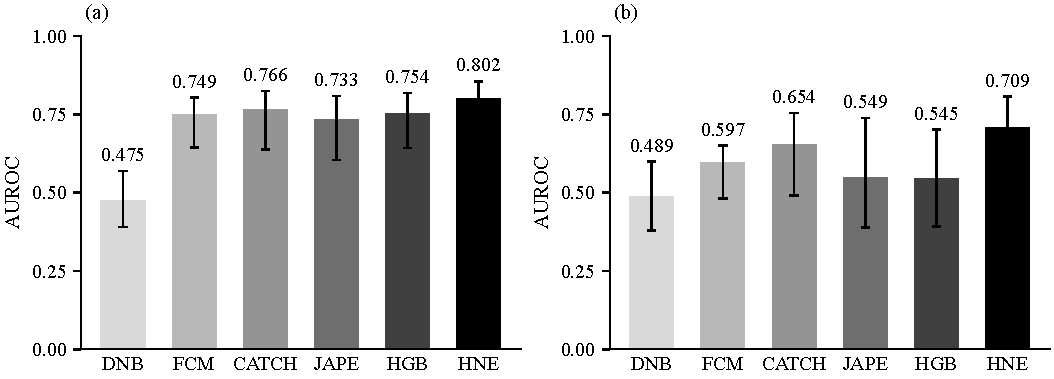
\includegraphics[width=\textwidth]{figures/main_auroc.pdf}
\caption{Development AUROC: (a) RESILIENT; (b) BrisT1D-Open. Error bars are participant-bootstrap 95\% intervals. JAPE uses validation-AUROC selection.}
\label{fig:main}
\end{figure*}





\subsection{Early Warning Performance}
\label{sec:results}
HNE leads the main comparison with AUROC $0.802$ on RESILIENT and $0.709$ on BrisT1D-Open (Table~\ref{tab:main}, Figure~\ref{fig:main}). Relative to CATCH, the strongest baseline, the paired gains are $0.036$ (95\% CI: $[-0.031,0.124]$) and $0.055$ ($[-0.024,0.162]$), respectively. Average precision also increases, from $0.358$ to $0.449$ on RESILIENT and from $0.211$ to $0.296$ on BrisT1D. The improvement therefore appears in both ROC and precision--recall performance; complete comparator-selection intervals are reported in Appendix~\ref{app:reproducibility}.




\subsection{RQ1: Multivariate Rhythm Precursors}
We compare three temporal scales and four descriptor classes using the same future labels and participant folds (Table~\ref{tab:temporal-ablations}). Combining scales raises BrisT1D AUROC from $0.685$ for the best single scale to $0.709$, whereas RESILIENT favors the eight-day window over the combined representation ($0.809$ versus $0.802$). The useful temporal scale therefore differs between cohorts.

\begin{table}[H]
\centering
\caption{Temporal scales and fluctuation descriptors under the same labels and participant folds.}
\label{tab:temporal-ablations}
\hnetable{tables/temporal_ablations}
\end{table}

Removing location, temporal-memory, or tail-frequency descriptors lowers AUROC in both cohorts. Amplitude descriptors improve RESILIENT, while their removal raises BrisT1D AUROC to $0.716$. The precursor signal therefore includes the persistence, displacement, and frequency of unusual observations. HNE exposes these distinct changes to the risk learner through the same multiscale coordinates.

\subsection{RQ2: Learning from History, Networks, and Context}

\begin{table}[H]
\centering
\caption{HNE module ablations on common origins. Human denotes Human Rhythms.}
\label{tab:ablations}
\hnetable{tables/modules}
\end{table}

Network coordinates add $0.024$ and $0.032$ AUROC on RESILIENT and BrisT1D, respectively (Table~\ref{tab:ablations}). These gains connect the warning task to changes in joint behavior: the predictor benefits from knowing how indicators move together relative to their personal reference. Environment adds $0.009$ on RESILIENT and reduces BrisT1D AUROC by $0.008$. On both cohorts, the conditional-reference construction outperforms direct context appending, supporting the design that encodes ordinary context responses alongside their departures.

\begin{table}[H]
\centering
\caption{Risk heads on the shared HNE representation.}
\label{tab:heads}
\hnetable{tables/heads}
\end{table}

Keeping the representation fixed, the additive predictor exceeds the evaluated boosting, set, temporal, and pairwise heads (Table~\ref{tab:heads}). Within-person AUROC is $0.541$ on RESILIENT and $0.629$ on BrisT1D, complementing the pooled evaluation.




\paragraph{Held-out cohorts.}
\begin{table}[H]
\centering
\caption{Held-out AUROC on 2,948 Human Rhythms and 14,963 College origins. Neural methods average three seeds.}
\label{tab:heldout}
\hnetable{tables/heldout}
\end{table}

\begin{table*}[t]
\centering
\caption{Frozen-source transfer. CARE and ESA use native fault and expert-event endpoints. Intervals resample people, assets, or spacecraft time blocks.}
\label{tab:transfer}
\hnetable{tables/crossdomain}
\end{table*}

HNE attains AUROC $0.603$ on Human Rhythms and $0.655$ on College, exceeding FCM and CATCH on both cohorts (Table~\ref{tab:heldout}). History HGB reaches $0.610$ and $0.668$, respectively; College JAPE also reaches $0.668$. HNE's strongest-control differences are $-0.007$ (95\% CI: $[-0.074,0.042]$) and $-0.012$ ($[-0.041,0.003]$).

The held-out module comparisons show distinct contributions: environment improves College and reduces Human Rhythms AUROC, while relationships show the reverse pattern. The common estimator therefore exposes different contributions from the available context and relationships. Source-data variants and operating points appear in the supplement.

\subsection{RQ3: Transfer Across Monitoring Domains}
\label{sec:transfer}




After source-only selection and fitting, the frozen rule transfers between the two development cohorts (Table~\ref{tab:transfer}). RESILIENT$\rightarrow$BrisT1D reaches AUROC $0.735$, and the reverse direction reaches $0.816$, exceeding source history-only scores of $0.698$ and $0.789$, respectively. Within-person scores are $0.571$ and $0.529$.



\paragraph{Transfer of the basis and coefficients.}
We compare target-only fitting, transfer of the source basis, and transfer of both the basis and source coefficients using 22, 43, or 85 Human Rhythms training participants. All conditions use the full HNE extractor, matched participants, and the same regularization candidates. Smaller budgets average three fixed subsets; validation and test participants remain unchanged.

\begin{figure}[H]
\centering
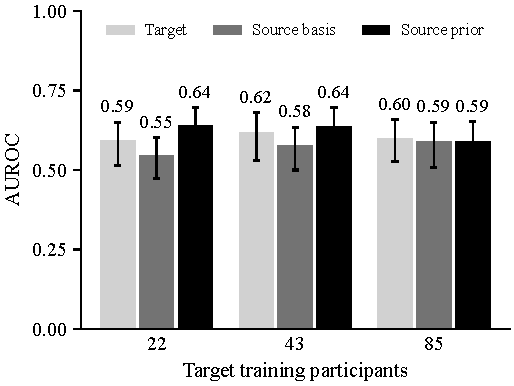
\includegraphics[width=\columnwidth]{figures/human_adaptation.pdf}
\caption{Effect of transferring the source basis and learned coefficients. Intervals jointly resample test participants across conditions and fixed training subsets.}
\label{fig:human-adaptation}
\end{figure}

At 22 participants, the source-coefficient prior reaches mean AUROC $0.639$, compared with $0.593$ for target-only fitting and $0.546$ for basis-only transfer (Figure~\ref{fig:human-adaptation}). Paired gains are $0.046$ (95\% CI: $[0.017,0.077]$) and $0.093$ ($[0.048,0.143]$). The basis-only control retains the source scaling and spline knots; adding the source coefficients supplies the learned link from those coordinates to future risk. This comparison identifies the warning rule itself as useful transferred information. Target-relative gains at 43 and 85 participants are $0.019$ and $-0.011$, respectively; complete budgets appear in Appendix~\ref{app:additional-results}.

\paragraph{Cross-domain endpoints.}
The unchanged extractor and human-source predictor also score industrial faults in CARE and expert-labelled spacecraft events in ESA. Relative to DNB on CARE, AUROC is $0.548$ versus $0.574$; relative to source history on ESA, it is $0.564$ versus $0.498$ on Mission 1 and $0.760$ versus $0.808$ on Mission 2. The Mission 1 gain is $0.066$ (95\% CI: $[-0.018,0.147]$), showing that transfer performance depends on the target domain and endpoint.


\subsection{Sensitivity to Observation Quality}
\label{sec:robustness}

\begin{figure*}[t]
\centering
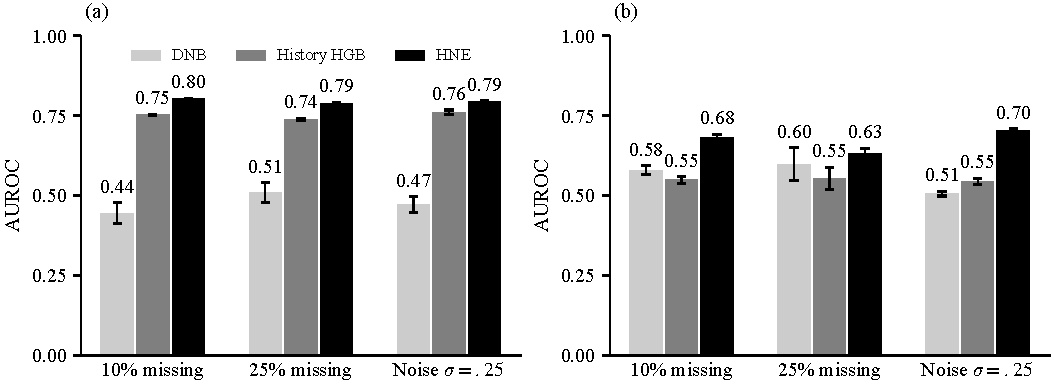
\includegraphics[width=\textwidth]{figures/robustness.pdf}
\caption{Observation perturbations: (a) RESILIENT; (b) BrisT1D-Open. Bars average three seeds, with seed standard deviations. All methods score common origins.}
\label{fig:robustness}
\end{figure*}




We perturb observed histories while holding the reference, future labels, and fitted models fixed. Figure~\ref{fig:robustness} compares HNE, History HGB, and DNB under 10\% or 25\% additional missingness and Gaussian noise of standard deviation $0.25$, averaging three seeds on common scoreable origins.

With 25\% additional missingness, HNE reaches AUROC $0.788$ on RESILIENT and $0.632$ on BrisT1D; under added noise, it reaches $0.795$ and $0.704$, respectively. BrisT1D is more sensitive to lost observations, while HNE retains the highest score among the three methods in each condition. Appendix~\ref{app:additional-results} reports all conditions; common-origin coverage at 25\% removal is 1,727--1,756 for RESILIENT and 1,195--1,206 for BrisT1D.

\section{Conclusion}
HNE turns changes in personal rhythms into a shared representation for future-disturbance warning. Personal deviations, context responses, and relationship changes retain the same coordinate definitions across different measurement sets. The main comparisons show gains in AUROC and average precision, with relationship changes strengthening warning on both cohorts. The source-coefficient experiment further identifies a concrete transfer benefit: learned warning rules improve low-data adaptation beyond transfer of the representation basis alone. HNE thus connects individual reference behavior, multivariate precursor signals, and learning across monitoring domains.

\section*{Limitations}
Estimating how an intervention changes disturbance risk requires interventional outcomes beyond the observational endpoint studied here. Relating wearable rhythm features to endogenous circadian phase requires independent phase measurements. These are two extensions of the present prediction task.

\section*{Impact Statement}
HNE supports research on longitudinal warning from physiological, behavioral, and operational records. Personal histories contain sensitive information, making controlled access and informed data use important. Warning systems also affect follow-up workload; application studies should evaluate alarm burden and decision consequences alongside predictive discrimination.

\bibliography{../literature/references}
\bibliographystyle{icml2026}

\appendix
\addtocontents{toc}{\protect\setcounter{tocdepth}{2}}
\renewcommand{\contentsname}{Appendix Contents}
\noindent\begin{minipage}{\columnwidth}
\tableofcontents
\end{minipage}\par
\section{Reproducibility Details}
\label{app:reproducibility}

\subsection{HNE Implementation}
Personal normalization requires 28 reference observations. Reference standard deviation replaces a zero median absolute deviation; constant variables remain unavailable. Context fitting requires at least 14 dates with the state and supported context observed. Missing context is zero-filled with its observation mask, and the intercept is unpenalized. Four contiguous 14-day reference blocks are each predicted from the other three blocks. Original normalized values replace residuals when context or fitting support is unavailable.

Each context coordinate at lags zero, one, and seven requires four reference observations and is clipped to $[-8,8]$ before concatenation with its observation mask. Context-response targets are clipped to $[-12,12]$ during reference fitting; the resulting residual stream uses the original normalized observations. Node descriptors require four window observations and 14 reference observations. Reference standard-deviation and amplitude denominators are floored at $0.1$ and $0.2$, respectively; the absolute-deviation tail threshold is floored at $0.1$. Population standard deviations and linearly interpolated quantiles are used throughout.

The $E$ group contains 104 pooled adjusted-state, coefficient-norm, and fitting-support coordinates plus 24 context descriptors averaged across context variables. Each of $N$ and $NE$ contains four graph summaries for three windows and three lags. For more than 32 state channels, the reference-only selection rule greedily maximizes coverage times one minus the largest absolute reference correlation with a selected channel. Eligible channels require 28 reference observations; source field names resolve exact ties. The quadratic spline expansion uses three uniform knots, linear extrapolation, and three retained bases per coordinate. Training standardization is applied before and after expansion.

Edges require six jointly observed pairs and nonzero variances in both periods. Zero-lag edges are unordered; lagged edges are directed and exclude self-edges. Risk-coordinate imputation uses training medians, followed by training mean/standard-deviation normalization and clipping to $[-8,8]$. Scaling each expanded group by $m_g^{-1/2}$ implements the group-weighted penalty through ridge logistic regression. Validation AUROC selects $C\in\{0.01,0.1,1\}$; single-class validation uses log loss.

\paragraph{Endpoint eligibility.}
Reference blocks require five observed days per variable and 20 qualifying blocks. A family is abnormal when any eligible member is abnormal, normal when all members are observed and normal, and otherwise unknown. A future block is positive with two abnormal families, negative when abnormal plus unknown families cannot reach two, and otherwise unlabelled. The preceding seven-day block must be known normal.

\begin{algorithm}[!tb]
\caption{Fit HNE and issue a prospective score}
\label{alg:hne}
\begin{algorithmic}[1]
\REQUIRE Training and validation people; daily states, context, masks; eligible origins and training endpoints
\FOR{each person $i$}
  \STATE $R_i\leftarrow\mathrm{FitReference}(X_{i,1:56},E_{i,1:56})$
  \STATE Fit context responses and four reference-block residual folds inside $R_i$
  \FOR{each eligible origin $d$}
    \STATE $z_{id}\leftarrow\mathrm{Encode}(R_i,X_{i,\leq d},E_{i,\leq d})\in\mathbb{R}^{296}$
  \ENDFOR
\ENDFOR
\FOR{$C\in\{0.01,0.1,1\}$}
  \STATE $f_C\leftarrow\mathrm{FitRisk}(z_{\mathrm{train}},y_{\mathrm{train}},C)$ using weighted spline logistic regression
\ENDFOR
\STATE Select $C$ on validation people; freeze imputation, scaling, basis, coefficients, and prior correction $\kappa$
\STATE For a monitored person, fit $R$ from the first 56 days
\STATE At issue time $d$, encode available observations only and return $\sigma(f_C(z_d)-\log\kappa)$
\end{algorithmic}
\end{algorithm}

\subsection{JAPE Interval-Event Adapter}
JAPE retains the released DSTR backbone, detached future-graph branch, 13-dimensional structural extractor, and dual-view alerting head. The backbone uses three layers, width 128, eight heads, FFN width 256, maximum lag three, and five graph predecessors; the alert head uses three layers, width 64, and four heads. Both stages use batch size 128, learning rate $10^{-4}$, at most 20 epochs, and patience five. Adam fits the backbone to summed main and auxiliary observed-entry MSE. With the backbone frozen, AdamW fits the alert head using weight decay $10^{-4}$, focal loss ($\alpha=0.25$, $\gamma=2$), and unit gradient clipping. Native selection maximizes validation F1 over 30 thresholds in $[0.05,0.95]$ and drives learning-rate reduction. Training-history medians fill inputs before training-only standardization; missing future values receive no supervision. Participant folds replace the original interleaved timeline split, and three fixed seeds are averaged. The adapter predicts interval events rather than pointwise anomalies or variable explanations.

The AUROC-selection condition retrains each alert head on its frozen forecaster, replacing validation F1 with AUROC for checkpoint selection and learning-rate reduction. All other settings remain fixed. Its 30 head fits and 306 epochs enter the extended strongest-control comparison alongside native F1 selection.

\subsection{Data Availability and Field Mapping}

\begin{table*}[!tb]
\centering
\caption{Cohort coverage and input dimensions. Units are available/scorable people or CARE assets; $P/Q$ are state/context dimensions. Span and Observed are median calendar and observed days; $n/n^+$ count eligible/positive origins.}
\label{tab:cohorts}
\hnetable{tables/cohorts}
\end{table*}

Table~\ref{tab:cohorts} summarizes recording coverage and dimensions. RESILIENT v3 is available from Zenodo under CC BY 4.0, with a companion data descriptor \citep{hneD02,hneD03}. We use its sleep-mat and smartwatch tables; 56 of the 73 available participants contribute eligible origins. BrisT1D-Open provides processed device records under CC BY 4.0 \citep{hneD04}. Its study recruited 24 participants; our device-data adapter contains 20, of whom 19 contribute eligible origins. CARE v6 provides 95 cases from 36 turbines under CC BY-SA 4.0: 45 fault-leading cases and 50 normal cases \citep{hneD05,hneD06}. These counts refer to the v6 release.

\begin{table}[H]
\centering
\small
\caption{Human-cohort fields before daily aggregation. Mean and standard-deviation coordinates inherit their source field's family.}
\label{tab:appendix-fields}
\begin{tabular}{@{}p{0.21\columnwidth}p{0.45\columnwidth}p{0.22\columnwidth}@{}}
\hline
Cohort & State fields & Families \\
\hline
RESILIENT & Sleep-mat and watch heart rate; respiration; SDNN; sleep proportion & Heart; respiration; HRV; sleep \\
BrisT1D & Glucose; heart rate; steps, distance, calories & Glucose; heart; activity \\
\hline
\multicolumn{3}{p{0.92\columnwidth}}{Context: step counts for RESILIENT; recorded carbohydrate intake for BrisT1D.} \\
\hline
\end{tabular}
\end{table}

Table~\ref{tab:appendix-fields} groups the measured states into endpoint families. Each state contributes a daily mean and population standard deviation from at least four observed hourly values; context requires one. Missing calendar positions remain explicit. Sleep proportion counts light, deep, and REM sleep by duration. RESILIENT uses UTC; BrisT1D retains its unspecified source timezone. Daily values become available at the following midnight.

Human Rhythms \citep{hneD07} supplies 166 participants with official daily heart-rate summaries, main-sleep summaries, and daily step summaries. The ten state coordinates are resting heart rate; sleep efficiency; minutes asleep, awake, in bed, to fall asleep, and after waking; steps; and the sine and cosine of main-sleep midpoint. The midpoint uses the actual recorded local start and end timestamps and is assigned to the sleep-end date. Heart, sleep, and activity are the three endpoint families. We retain only step segments explicitly marked daily with full-day boundaries; weekly, multiday, and whole-trajectory fitted rhythm files do not enter features. Five context fields are mean air temperature, relative humidity, precipitation, wind speed, and daylight duration from the study-location weather table. Calendar gaps remain missing.

IDs are ordered by SHA-256 of \texttt{20261110:Human-Rhythms:}\textit{ID}; the first 100, next 33, and final 33 form training, validation, and test. Outcomes and coverage do not influence this allocation. Native daily records are aligned to the following local midnight in our retrospective protocol. The source weather consists of historical site-level estimates; its original publication latency is not supplied, so this alignment is an analysis convention rather than a verified real-time feed. The dataset's published rhythm analyses do not provide future-disturbance event labels; our fixed endpoint constructs those labels from subsequent observations.

CARE uses documented non-angle, non-counter average fields, yielding 78/102/438 daily state coordinates in farms A/B/C before the common 32-coordinate reference-based selection. Its 3/5/7 context coordinates measure wind speed, ambient or outside temperature, and, in farm C, external air pressure. Cases remain separate because their years were anonymized independently. Within the published prediction segment, a positive origin has an official fault boundary in $[\mathrm{issue}+1,\mathrm{issue}+8)$ days. Negatives require follow-up through the right endpoint; gap failures and post-failure origins are excluded. Normal-case interval ends are not faults. Event annotations and operating-status labels are excluded from features. This native endpoint does not require the human cohorts' two-family condition.

\paragraph{TOLIFE coverage.}
We also apply the unchanged physiological field mapping and fluctuation protocol to all 17 originally reserved TOLIFE participants \citep{hneD01}. Their 4,041 calendar days contain 2,635 candidate origins but no eligible normal-start window: preceding-week labels remain unknown under the observation requirements. This cohort contributes a coverage result, not a test AUROC.

\subsection{Released Neural Baselines and Score Adaptation}
Released FCM and CATCH cores \citep{hneH01,hneC01} are pinned to commits \texttt{67e4c84} and \texttt{3647c69}. Development inputs are $32\times11$ histories, imputed with training-channel medians and standardized on training histories. Both methods complete 20 epochs at batch size eight for seeds 20261110--20261112: 60 fits and 1,200 epochs across cohorts and folds. Training uses an RTX 4060 Laptop GPU and PyTorch 2.8.0+cu128. FCM has 831,243 parameters; CATCH has 1,111,840.

Human Rhythms uses $32\times15$ inputs and six additional 20-epoch fits. FCM fits 7,654/2,099 training/validation origins with 32 complete calendar days of future supervision; incomplete tails are excluded only from fitting. CATCH fits all 9,039/2,526 histories. Both subsequently score all eligible histories. The test feature archive contains no future trajectories.

FCM uses four layers, eight heads, and model/FFN widths 128/128. It retains reconstruction, association-minimax, and future-context objectives, with Adam rate $10^{-3}$, association coefficient 3, and scoring temperature 50. The context branch activates after epoch one; predicted context is detached while its projection receives gradients. Validation forecast MSE selects the checkpoint after activation. Inference sums KL-weighted history reconstruction energy with predicted future context.

CATCH retains full FFT, frequency patches, channel masks, and bilevel updates. It uses three layers, two heads, widths 64/128, patch length 16, and stride eight. Main/mask Adam rates are $10^{-4}/10^{-5}$; frequency and discovery coefficients are both 0.005. Validation reconstruction MSE selects the checkpoint. Scores average temporal reconstruction error plus 0.05 times the frequency criterion. Validation and inference use fixed Gumbel streams.

Neither encoder is trained on event labels. The separate \emph{score-LR} condition fits standardized scalar-score logistic regression on training events, selecting $C\in\{0.01,0.1,1\}$ by validation log loss. For each fold and seed, the ensemble transform is $F_s(a)=\#\{v:y_v=0,a_v\leq a\}/\#\{v:y_v=0\}$. The three frozen validation-negative transforms are averaged equally on every partition. Thus event labels calibrate the ensemble scores while encoder objectives remain unchanged.

\subsection{DNB and MM-DEV}
DNB uses normalized states from the last 32 days. Among the ten highest-coverage channels, it chooses the largest feasible set of five, four, or three channels, preferring joint coverage, requiring 12 complete observations and nonzero variances. Within that set, it maximizes
\begin{equation}
 D(M)=\frac{\overline{\mathrm{SD}}_M\,
 \overline{|\rho|}_{M,M}}{\overline{|\rho|}_{M,M^c}+10^{-6}}
\end{equation}
over two- and three-channel modules with a nonempty complement. Undefined windows remain missing. DNB-tuned selects among 16-, 24-, and 32-day histories by validation AUROC.

The daily MM-DEV adaptation retains ISOMAP, mixed embedding, S-map Jacobians, and dominant-eigenvalue scoring \citep{hneM10}. Each 32-day, 11-coordinate history is median-filled and standardized independently; constant coordinates are dropped. ISOMAP uses a symmetric five-neighbor graph and up to three positive manifold coordinates. A disconnected graph yields an undefined score. Embedding dimension $E\in\{1,\ldots,6\}$ maximizes leave-one-out, one-step prediction correlation of the first coordinate with $\theta=0$; ties favor smaller $E$. Mixed embeddings use contemporaneous manifold coordinates followed by first-coordinate lags. The final 24 embedded days provide S-maps with delay one and $\theta=1$. Each local regression excludes its focal transition and multiplies both sides by exponential distance weights. The score is the mean dominant-eigenvalue modulus. All fitting uses the observed history, unlike fitting ISOMAP once to a complete trajectory. Its separate score-LR uses HNE's participant/class weights and validation AUROC selection.

\subsection{Inference Cost}
We measure loaded-model CPU time on 128 uniformly sampled Human Rhythms test origins, using one i9-13900HX thread, batches of eight, and five repeated calls after initialization. Inputs are already normalized histories. HNE includes per-origin coordinate extraction and repeated context-reference fitting; history boosting includes its descriptors, and the neural ensembles include all three seeds, imputation, scaling, and score transforms. Data/model loading and common initial normalization are excluded. HNE requires a median 31.49 ms per origin; its separately timed cached-coordinate head takes 1.50 ms. Table~\ref{tab:inference-cost} reports the complete measured scope for each method.

\begin{table}[!htb]
\centering
\caption{CPU inference time and saved predictor size. IQR is the spread over five timed calls. Cached-head timing excludes coordinate construction.}
\label{tab:inference-cost}
\hnetable{tables/inference_cost}
\end{table}

\subsection{Statistical Definitions}
For evaluation fold $k$, let $n_k^+$ and $n_k^-$ count positive and negative origins. The development estimate
\begin{equation}
 \widehat{\mathrm{AUC}}=
 \frac{\sum_k n_k^+n_k^-\widehat{\mathrm{AUC}}_k}
 {\sum_k n_k^+n_k^-}
\end{equation}
compares scores within each fitted model. Its common population requires finite DNB, FCM, CATCH, History-LR, History-HGB, HNE-HGB, and HNE-additive scores; additional methods retain their own coverage. Paired comparisons use the shared origins. Percentile intervals use 2,000 participant resamples (seed 20261110), retaining complete personal timelines and identical draws across methods. Within-person AUROC averages people with both classes. Alarms strictly exceed validation-negative 90th percentiles; average precision pools scores transformed by each fold's validation-score empirical CDF. CARE resampling clusters cases by farm-specific turbine identity.

Reselecting the strongest development comparator in each draw gives gain intervals $[-0.037,0.070]$ for RESILIENT and $[-0.105,0.113]$ for BrisT1D. The external primary set is HNE, DNB, daily MM-DEV, History-LR, History-HGB, and three-seed FCM/CATCH. DNB scores 2,948 of 2,980 Human Rhythms origins; the other primary methods score all origins. Their intersection contains 448 positives and 2,500 negatives. Each method has one frozen scoring function, so external metrics use global AUROC and direct average precision. Each strongest-control draw subtracts the maximum AUROC of the six controls from HNE's score; paired intervals instead retain a fixed comparator.

Human Rhythms sample-efficiency subsets select 22 or 43 of the 85 eligible training people by fixed ID hashes with seeds 20261110--20261112, independently of outcomes. Conditions share subsets and the complete validation/test sets. Estimates average the three subset-specific metrics; joint test-participant resampling applies identical weights across all conditions and subsets before averaging. These intervals measure test-participant uncertainty for the three fixed training subsets. The 85-person target-only condition is the primary target-trained HNE model.

\subsection{Context and Future-Block Sensitivity}
The primary context-response ridge coefficient is 10. A separate grid selects this coefficient from $\{0.1,1,10\}$ jointly with $C\in\{0.01,0.1,1\}$ by validation AUROC. Only the context-adjusted coordinates change; the raw history and relation coordinates remain identical. Human Rhythms selects ridge $0.1$ and $C=0.01$. The pooled-domain model uses the same nine candidates and the same Human Rhythms validation set, selecting the same pair. It fits on 12,267 origins from 160 eligible training participants across the three cohorts, with equal domain weights.

The forecast-distance comparison in Appendix~\ref{app:additional-results} moves the future seven-day block to gaps of one, three, or seven complete days while keeping every fitted model unchanged. It retains only origins whose labels are known at every evaluated gap. This measures ranking for progressively more distant intervals, rather than estimating the exact onset time of a clinical event. Both aggregate and within-person AUROC are reported to separate stable between-person risk from temporal discrimination.



\section{Additional Warning Comparisons}
\label{app:additional-results}

\subsection{Development Controls and Alarm Operating Points}
DNB tuning and daily MM-DEV probe whether the development ranking follows from the choice of a particular baseline window or score mapping. Table~\ref{tab:additional-baselines} reports each method on its scoreable origins; the main comparison in Section~\ref{sec:results} uses only origins scored by all primary methods.
\begin{table}[!htb]
\centering
\caption{Additional controls on their scored origins within the primary evaluation population.}
\label{tab:additional-baselines}
\hnetable{tables/additional_baselines}
\end{table}

Table~\ref{tab:operating-points} converts ranking performance into alarm operating points. Each threshold is the 90th percentile of validation-negative scores, applied unchanged to evaluation origins. TPR measures detected positive intervals and FPR measures alarms among normal intervals.
\begin{table}[!htb]
\centering
\caption{Development operating points at validation-selected thresholds. FCM/CATCH here use individual-seed scores.}
\label{tab:operating-points}
\hnetable{tables/operating_points}
\end{table}

At the fixed operating point, HNE detects 46.0\% of positive RESILIENT intervals versus 35.2\% for CATCH, with false-positive rates of 12.4\% and 12.2\%. On BrisT1D, detection rises from 25.1\% to 32.9\% while false positives fall from 12.9\% to 11.3\%. The ranking gains therefore also produce more detected events at these validation-selected thresholds.

\subsection{Human Rhythms: Complete Comparison}
Table~\ref{tab:external-main} gives all discrimination and alarm metrics on the same 2,948 test origins. HNE reaches AUROC $0.603$, compared with $0.547$ for FCM and $0.542$ for CATCH; History HGB reaches $0.610$. Pairing each comparison on the same participants separates model differences from observation coverage.
\begin{table}[!htb]
\centering
\caption{Human Rhythms on 2,948 common test origins. Neural methods average three seeds; TPR/FPR use validation-negative 90th-percentile thresholds.}
\label{tab:external-main}
\hnetable{tables/external_main}
\end{table}

\paragraph{Representation and source data.}
Table~\ref{tab:external-variants} compares changes to the representation and the use of source data. The context grid selects the reference regression strength on validation people; frozen-source and pooled-domain models add source information through different fitting routes. Each scores the same target origins.
\begin{table}[!htb]
\centering
\caption{Human Rhythms representation and source-data variants.}
\label{tab:external-variants}
\hnetable{tables/external_variants}
\end{table}

The source-data conditions distinguish two routes to better target scores. Frozen-source HNE reaches AUROC $0.663$ without target fitting; pooled-domain training reaches $0.675$, compared with $0.603$ for target-only HNE. Selecting the context-reference strength separately reaches $0.639$. These controls locate the changes in the training population and reference fit while retaining the shared coordinate definitions.

\paragraph{Neural scores and supervised readout.}
Table~\ref{tab:external-seeds} separates individual seeds from the supervised scalar readout of each frozen encoder. The readout learns a score-to-event mapping from training people; the encoder remains fixed. The main comparison averages all three predetermined neural seeds.
\begin{table}[!htb]
\centering
\caption{Human Rhythms seeds. Each cell reports native / supervised scalar-readout scores.}
\label{tab:external-seeds}
\hnetable{tables/external_seeds}
\end{table}

\FloatBarrier
\subsection{Target-Sample Budgets}
Table~\ref{tab:human-adaptation} reports the complete Human Rhythms sample-efficiency comparison. At 22 training people, the source-coefficient prior improves AUROC by $0.046$ over target-only fitting and $0.093$ over basis-only transfer. The 43- and 85-person conditions track how that advantage changes as target data grow.
\begin{table}[!htb]
\centering
\caption{Human Rhythms AUROC by target-training budget. Smaller budgets average three fixed subsets.}
\label{tab:human-adaptation}
\hnetable{tables/human_adaptation}
\end{table}

CARE repeats the adaptation comparison with six or eleven training assets per fold, corresponding to 25\% and 50\% of the available assets (Table~\ref{tab:care-adaptation}). The target-only, source-basis, and source-prior conditions share the same asset subsets and evaluation folds.
\begin{table}[!htb]
\centering
\caption{CARE adaptation with matched training-asset budgets.}
\label{tab:care-adaptation}
\hnetable{tables/care_adaptation}
\end{table}

The source-prior advantage over target-only fitting is $0.041$, $0.018$, and $0.020$ at the three asset budgets. At the smallest budget, source-basis transfer alone reaches $0.548$, slightly above the coefficient prior's $0.546$. At the two larger budgets, adding the coefficient prior improves on basis transfer by $0.011$ and $0.013$. The matched conditions separate transferable scaling from the learned risk coefficients.

\subsection{Forecast Distance and Observation Quality}
Table~\ref{tab:lead-time} evaluates the same fitted predictor at one-, three-, and seven-day gaps before the seven-day target interval. Each comparison retains origins labelable at all gaps, exposing how forecast distance changes ranking while holding the fitted model fixed.
\begin{table}[!htb]
\centering
\caption{Seven-day target intervals at three forecast gaps. Models are frozen from the one-day-gap task.}
\label{tab:lead-time}
\hnetable{tables/lead_time}
\end{table}

RESILIENT AUROC stays between $0.810$ and $0.825$ across the three gaps, exceeding CATCH at each distance. BrisT1D falls from $0.720$ to $0.663$ as the gap increases, while remaining above CATCH. The same frozen rule thus retains useful ranking at longer horizons, with the size of the change determined by the cohort.

Table~\ref{tab:robustness} reports every perturbation score. Additional missingness is applied to state and context observations, and noise is added in normalized units; the reference and future endpoint remain fixed. The standard deviations summarize the three predetermined perturbation seeds.
\begin{table}[!htb]
\centering
\caption{Observation perturbations: AUROC mean and standard deviation over three seeds.}
\label{tab:robustness}
\hnetable{tables/robustness}
\end{table}


\section{College Participant-Held-Out Evaluation}
\label{app:college-test}
\newcommand{\CollegeN}{14963}
\newcommand{\CollegePeople}{41}
\newcommand{\CollegeAllN}{15137}
\newcommand{\CollegePositive}{4074}
\newcommand{\CollegeHNE}{0.655}
\newcommand{\CollegeFCM}{0.606}
\newcommand{\CollegeCATCH}{0.581}
\newcommand{\CollegeBestName}{History HGB}
\newcommand{\CollegeBestAUC}{0.668}
\newcommand{\CollegeBestDelta}{-0.012}
\newcommand{\CollegeBestLow}{-0.041}
\newcommand{\CollegeBestHigh}{0.003}
\newcommand{\CollegeDelayedFrozen}{0.655}
\newcommand{\CollegeDelayedIntercept}{0.667}
\newcommand{\CollegeDelayedAffine}{0.667}
\newcommand{\CollegeDelayedCoefficients}{0.667}
\newcommand{\CollegeDelayedBestName}{History HGB / intercept}
\newcommand{\CollegeDelayedBestAUC}{0.683}

College Experience v5 contains 220 identifiers, assigned by a fixed hash to 132/44/44 training/validation/test participants \citep{hneD08}. Nine states describe phone-derived sleep, stationary and vehicle duration, cycling and walking, phone unlock duration and count, travel distance, and visited locations. Four contexts describe home, study and social duration, and campus distance. Phone-derived sleep and phone use share one measurement family; activity and mobility form the other two. The same 56-day reference, 32-day history, one-day gap, and seven-day target yield 54,691/19,876 training/validation origins from 126/44 eligible people.

The 44 participants reserved at the initial identifier split enter evaluation only after all selected models are frozen. The fixed event protocol yields \CollegeAllN{} origins from \CollegePeople{} eligible participants, including \CollegePositive{} positives. The primary comparison uses \CollegeN{} origins scoreable by every prespecified control. As in Human Rhythms, confidence intervals resample participants, and the strongest comparator is selected again within each bootstrap draw.

\begin{table}[!htb]
\centering
\caption{College prediction on 14,963 common test origins. Within is mean within-participant AUROC; TPR/FPR use validation-selected thresholds.}
\label{tab:college-test}
\hnetable{tables/college_test}
\end{table}

Table~\ref{tab:college-test} reports the complete primary comparison. HNE reaches AUROC \CollegeHNE{}, compared with \CollegeFCM{} for FCM and \CollegeCATCH{} for CATCH. The strongest prespecified comparator is \CollegeBestName{} at \CollegeBestAUC{}; HNE's difference is $\CollegeBestDelta$ with paired interval $[\CollegeBestLow,\CollegeBestHigh]$.

\FloatBarrier
Table~\ref{tab:college-test-variants} isolates the representation groups on the same test origins. Full HNE reaches AUROC $0.655$ versus $0.647$ for history alone; removing network or environmental coordinates gives $0.663$ and $0.638$, respectively.

\begin{table}[!htb]
\centering
\caption{College representation ablations on the common test population.}
\label{tab:college-test-variants}
\hnetable{tables/college_core_variants}
\end{table}

\subsection{Source-Rule Adaptation}
The fixed source-basis and source-prior experiment repeats the Human Rhythms design with 32, 63, and all 126 eligible College training participants. The two smaller budgets each use three predetermined identifier subsets; validation and test participants remain the same across conditions. Table~\ref{tab:college-adaptation} reports the mean AUROC across these fixed subsets.

\begin{table}[!htb]
\centering
\caption{College transfer at fixed target-training budgets.}
\label{tab:college-adaptation}
\hnetable{tables/college_adaptation}
\end{table}

\subsection{Learning from Matured Personal Outcomes}
The prequential experiment exposes the same delayed feedback to every method. At issue day $d$, only outcomes originating at $s\le d-8$ can update the predictor. Updates use a 90-day memory, occur every seven days, and require at least eight matured origins. Intercept and positive-affine updates recalibrate the frozen score; HNE also permits source-regularized updates to its spline coefficients. Native public scores receive a training-participant logistic readout before the same calibration experiment.

\begin{table}[!htb]
\centering
\caption{College prequential AUROC with matched availability of matured outcomes. Coefficient updates apply to HNE spline models.}
\label{tab:college-delayed}
\hnetable{tables/college_delayed}
\end{table}

Frozen HNE, intercept adaptation, affine adaptation, and coefficient learning reach AUROC \CollegeDelayedFrozen{}, \CollegeDelayedIntercept{}, \CollegeDelayedAffine{}, and \CollegeDelayedCoefficients{}, respectively (Table~\ref{tab:college-delayed}). The highest point estimate among all declared conditions is \CollegeDelayedBestAUC{} for \CollegeDelayedBestName{}. These evaluations follow one fixed learning rule through the held-out participants' timelines; their feedback regime is separate from the static primary comparison.


\section{Spacecraft Transfer with Expert Event Labels}
\label{app:esa}

\subsection{Telemetry and Future Event Labels}
ESA-AD v2 supplies long spacecraft telemetry, executed-command logs, and expert event annotations \citep{hneD09,esaADv2}. We aggregate observed hourly means into daily means and standard deviations for numerical target channels. Numerical non-target channels and four command-priority counts provide context. Missions 1 and 2 contribute 5,114/1,277 published-clock days, 116/94 state coordinates, and 22/47 context coordinates before the unchanged reference-based 32-state budget. Their clocks are anonymized and scaled; the reported time units are not physical days.

The original initial-reference fluctuation endpoint produces no eligible training/validation origins on either mission: all 2,462/544 candidate origins have an already abnormal preceding week. We evaluate a separately defined expert endpoint, fixed before the Mission 2 analysis, without changing HNE's features or risk function. A positive origin precedes the earliest onset of an event labelled multivariate and subsequence by one to seven complete days. The preceding seven days contain no expert anomaly, and the intervening day contains no anomaly onset. Future univariate or point anomalies are excluded from the negative class. Expert-labelled rare normal events remain negative examples. Labels never enter the historical features.

Mission 1 training ends before October 2006, validation occupies the following three months, and testing begins in January 2007. Its training/validation populations contain 1,875/40 origins and 224/4 positives. Mission 2 uses July and October 2001 boundaries, yielding 304/85 training/validation origins and 55/0 positives. The shared selection function uses validation log loss when AUROC is undefined; FCM and CATCH retain their native validation losses. All twelve public-model runs complete 20 epochs. Frozen testing yields 2,007/566 origins and 230/14 positives for Missions 1/2. Uncertainty resamples 64-day blocks jointly across methods; observations within one spacecraft are not treated as independent systems.

\subsection{Frozen Source Rules}
On Mission 1's 2,007 shared source-transfer origins, source HNE reaches AUROC .564, compared with .498 for source history and .490 for DNB (Table~\ref{tab:esa-source}). Mission 2 gives .760/.808/.123 on 566 origins. 

\begin{table}[!htb]
\centering
\caption{Frozen human-source rules on ESA expert events. Thresholds use validation-negative percentiles.}
\label{tab:esa-source}
\hnetable{tables/esa_source}
\end{table}

\subsection{Target-Domain Training}
Target-domain fits are a separate comparison: on 1,980/469 common origins, target HNE reaches .555/.346, FCM .504/.449, and CATCH .445/.508. The strongest target controls are history logistic regression at .591 on Mission 1 and history boosting at .730 on Mission 2 (Table~\ref{tab:esa-target}). Source history exceeds full source HNE on Mission 2, reversing their ordering on Mission 1.

\begin{table}[!htb]
\centering
\caption{ESA target-trained models on common origins. Neural methods average three seeds; intervals resample 64-day blocks.}
\label{tab:esa-target}
\hnetable{tables/esa_target}
\end{table}

\subsection{Rare Normal Events}
On Mission 1, rare normal events overlap 292 negative test windows. Source HNE's false-positive rate is 43.5\% in these windows and 43.1\% in the other 1,485 negative windows; source history gives 49.3\% and 49.4\%, respectively (Table~\ref{tab:esa-benign}). Every one of Mission 2's 552 negative windows overlaps a rare normal event; source HNE and source history yield false-positive rates of 3.8\% and 2.2\%. Mission 2 therefore supplies no ordinary-negative subgroup for the same within-mission contrast.

\begin{table}[!htb]
\centering
\caption{False alarms during expert-labelled rare normal events and other negative windows. Thresholds are fixed before testing.}
\label{tab:esa-benign}
\hnetable{tables/esa_benign}
\end{table}

\section{Further Wearable Transfer}
\label{app:ssaqs}

\subsection{SSAQS: Student Wearable Records}
The 2026 release contains 35 students, including 32 with wearable records \citep{hneD10}. Observed-day medians are 60.5 for HRV, 51.5 for sleep, and 90.5 for steps. Ten states cover HRV summaries, sleep score and deep-sleep duration, and reported stress and anxiety. Six contexts comprise steps, four activity fractions, and course schedules. Questionnaires enter on their local completion day. Oxygen measurements without artifact flags and the composite Fitbit stress score are excluded. Twelve participants contribute 154 eligible origins and 19 positives; the six-method intersection retains all positives. Table~\ref{tab:ssaqs} compares the frozen rules. HNE reaches .867 AUROC on all origins and .819 on common origins, versus .823 for source history. Its strongest-control difference is $-.004$ [$-.166,.005$]. Only three participants have both outcome classes; HNE's within-participant AUROC is .499.

\begin{table}[H]
\centering
\caption{Frozen-source wearable transfer. SSAQS uses 118 origins from 11 people; PMData uses 404 from 14. Within is mean within-participant AUROC.}
\label{tab:ssaqs}
\hnetable{tables/ssaqs_transfer}
\end{table}

\subsection{PMData: Daily Activity and Wellness}
PMData records 16 participants over five months \citep{pmdata2020}. We reuse the available official daily files, retaining 11 states across sleep, resting heart rate, and wellness reports, with four activity-duration contexts. Calendar spans are 141--152 days. Fourteen participants contribute 509 origins and 36 positives. Seven methods jointly score 404 origins and 29 positives. HNE reaches .428 AUROC on all origins and .411 on common origins, versus .487 for DNB. Its strongest-control difference is $-.076$ [$-.489,.016$]. Figure~\ref{fig:ssaqs} contrasts both wearable cohorts. PMData reuses previously examined source records under the shared endpoint.

\paragraph{Shared inference.}
Both cohorts retain the 56/32/1/7-day reference/history/gap/future protocol. HNE and history-only reuse the RESILIENT+BrisT1D source models. Tree controls use the same source people and either 96 history or all 296 coordinates, with domain-balanced weighting and source-only regularization selection. No model is fitted on either target cohort. DNB and MM-DEV use their existing daily implementations; PMData additionally includes past-only CNM-GC. Intervals use 2,000 complete-participant resamples and reselect the strongest control within each draw.

\begin{figure}[H]
\centering
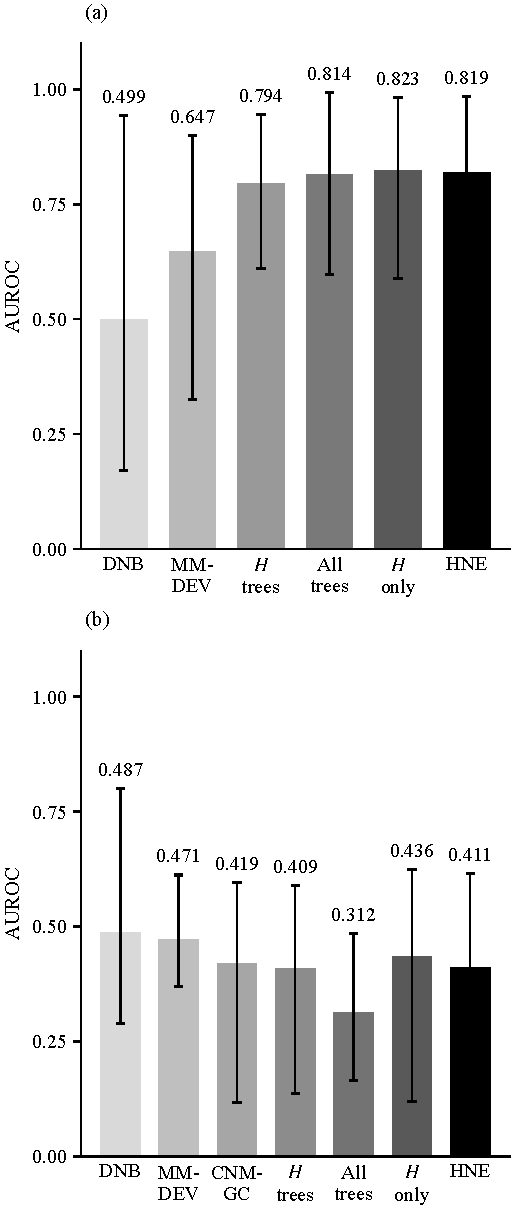
\includegraphics[width=\columnwidth]{figures/ssaqs_transfer.pdf}
\caption{Frozen-source AUROC on (a) SSAQS and (b) PMData. Error bars are participant-bootstrap intervals.}
\label{fig:ssaqs}
\end{figure}


\end{document}
